Before we discuss how BitShares achieves price \emph{stability}, we first need
to define what properties make a currency \emph{stable}.

In the U.S. for instance, the Federal Reserve (FED) has a mandate of
\emph{stable prices} and it is almost universally accepted by the market that
this is a good mandate. The same holds true for the Euro, with its stability
being achieved through the European Central Bank (ECB). Almost every country
applies a similar methods to gain control over prices via monetary policies
like quantitative easing and fixing of the interest rates for commercial banks
that borrow money from the central bank.

As a very basic example, imagine that a central bank has managed to keep prices
stable through their monetary policy with 0\% price inflation for 20 years.
Now let's assume that during this same 20 years the advances in robotics and
automation resulted in a 3x increase in efficiency and thus there are now 3x as
much food, cars, phones, houses, etc. For the sake of this example we will
assume the population is the same and everyone has the same amount of money in
the bank. You would normally expect that everything would be 1/3 the price and
that everyone would be able to afford 3x their prior lifestyle. However, this
is unfortunately not the case. Because of constant intervention by the central
banks, they have managed to also increase the money supply by 3x. The newly
created money is then lent to the commercial banks which then lend it again to
the people at a profit.

Since this monetary inflation results in a sustained increase in the general
level of prices, it is equivalent to a decline in the purchasing power of
money. Hence, a dollar buys less and less over time. As a result, we see the
dollar hast lost 99\% of its \emph{purchasing power} since the FED was founded
in 1913~(see \cref{fig:monetarybase}). 

\begin{figure}[!htp]
 \centering
 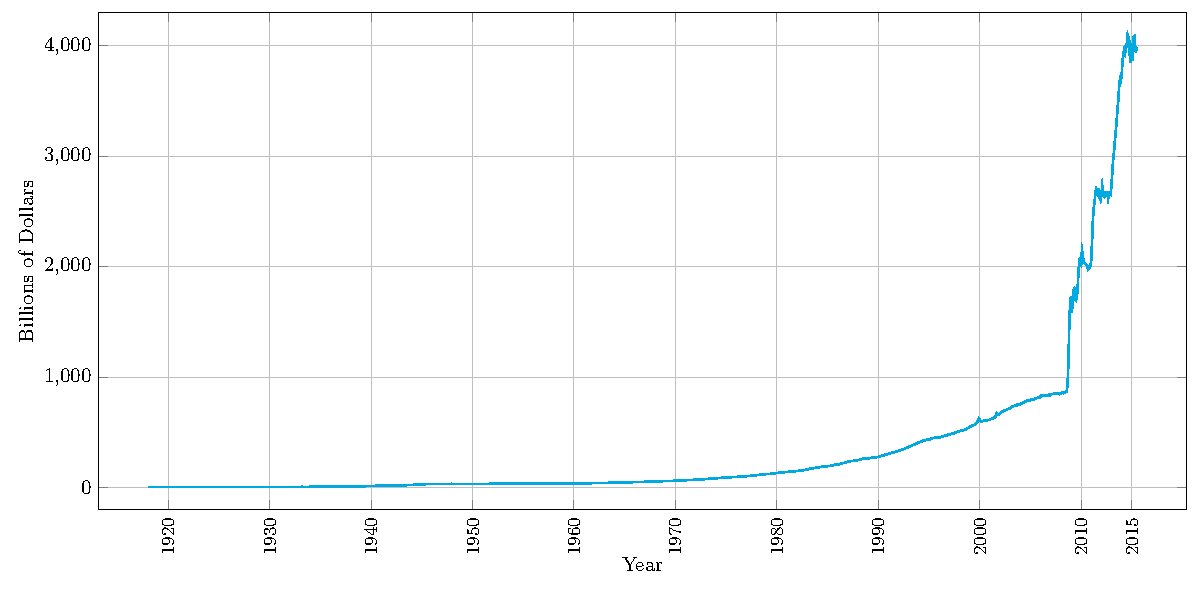
\includegraphics[width=\linewidth]{figures/monetary-base}
 \caption{St. Louis Adjusted Monetary Base~\cite{ambsl}}
 \label{fig:monetarybase}
\end{figure}

Of course, the goal of this paper is not to propose a replacement for central
banks or their monetary policies, but we do wish to clarify some terminology,
particularly as it relates to other ``stable'' cryptocurrencies. Other projects
in the cryptocurrency space have attempted to provide an alternative currency
that will ultimately achieve a similar mandate as the central banks, leaving
the profits in the hands of only few institutional entities. BitShares
\emph{market-pegged} assets will not result in the centralization of power and
control in this way.

Let us discuss the example above. Since the centralized bank policies have
resulted in a steady decrease in purchasing power over time, we notice that
price stability does not seem very important to them. Eventually, the ideal
goal would be to achieve a currency with a long term \emph{stable purchasing
power}. However, for now we must be content to achieve \emph{relative
stability} by pegging SmartCoins to the dollar or euro or gold, etc. To
summarize, what we want to achieve is:
\begin{itemize}
 \item a \emph{predictable} price with \emph{reduced volatility}
 \item a somewhat reliable ability to \emph{predict the future value} of a token, and
 \item a unit of account that doesn't have any meaningful capital gains or
       losses for tax purposes.
\end{itemize}

Hence for us, price ``stability'' means price \emph{predictability} within some
tolerance level. In the case of the U.S. dollar, a willingness to accept a
yearly loss in purchasing power via monetary policies demonstrates that
predictability is more important than stability~\cite{bm:stable:impossible}.

Alternatively, BitShares offers a decentralized solution to implement the
Consumer Price Index (CPI) to peg to the changes in the price of a market
basket of goods and services purchased by regular households. This is another
way BitShares users can hold and trade a stable crypto token that will help
them retain their purchasing power.
